\documentclass[hyperref]{ctexart}

\usepackage[left=2.50cm, right=2.50cm, top=2.50cm, bottom=2.50cm]{geometry} %页边距
\usepackage{helvet}
\usepackage{amsmath, amsfonts, amssymb} % 数学公式、符号
\usepackage[english]{babel}
\usepackage{graphicx}   % 图片
\usepackage{url}        % 超链接
\usepackage{bm} 
%\usepackage{graphicx}        % 加粗方程字体
\usepackage{multirow}
\usepackage{booktabs}
\usepackage{algorithm}
\usepackage{algorithmic}
\renewcommand{\algorithmicrequire}{ \textbf{Input:}}       
\renewcommand{\algorithmicensure}{ \textbf{Initialize:}} 
\renewcommand{\algorithmicreturn}{ \textbf{Output:}}     
%算法格式
\usepackage{fancyhdr} %设置页眉、页脚
\pagestyle{fancy}
\chead{{\Large \textbf{说\hspace{1em}明\hspace{1em}书}}}
\cfoot{\thepage}
%\usepackage{hyperref} %bookmarks
\hypersetup{colorlinks, bookmarks, unicode} %unicode
\usepackage{multicol}
\usepackage{indentfirst} %%缩进

% 专利发明名称
\newcommand{\name}{一种猫咪投币算法}

\newcommand{\applypublicnumber}{123123123}
\newcommand{\applypublicdate}{\the\year~年~\the\month~月~\the\day~日}
\newcommand{\applynumber}{123123123}
\newcommand{\applydate}{\the\year~年~\the\month~月~\the\day~日}
\newcommand{\proposer}{XXXX大学}
\newcommand{\authoraddress}{XX市XX区XX街道XX路XX号}
\newcommand{\patentauthor}{XXX \hspace{1} XXXX}
%封面摘要部分
\newcommand{\coverabstract}{
    \begin{large}
        猫,属于猫科动物,分家猫、野猫,是全世界家庭中较为广泛的宠物。家猫的祖先据推测是古埃及的沙漠猫,
        波斯的波斯猫,已经被人类驯化了3500年(但未像狗一样完全地被驯化)。一般的猫:头圆、颜面部短,
        前肢五指,后肢四趾,趾端具锐利而弯曲的爪,爪能伸缩。夜行性。以伏击的方式猎捕其它动物,大多能攀援上树
        猫的趾底有脂肪质肉垫,以免在行走时发出声响,捕猎时也不会惊跑鼠。行进时爪子处于收缩状态,防止爪被磨钝,
        在捕鼠和攀岩时会伸出来
    \end{large}
    \newline
    \newline\\
    \newline\\
    \newline
    \begin{figure}[H]
        \begin{center}
            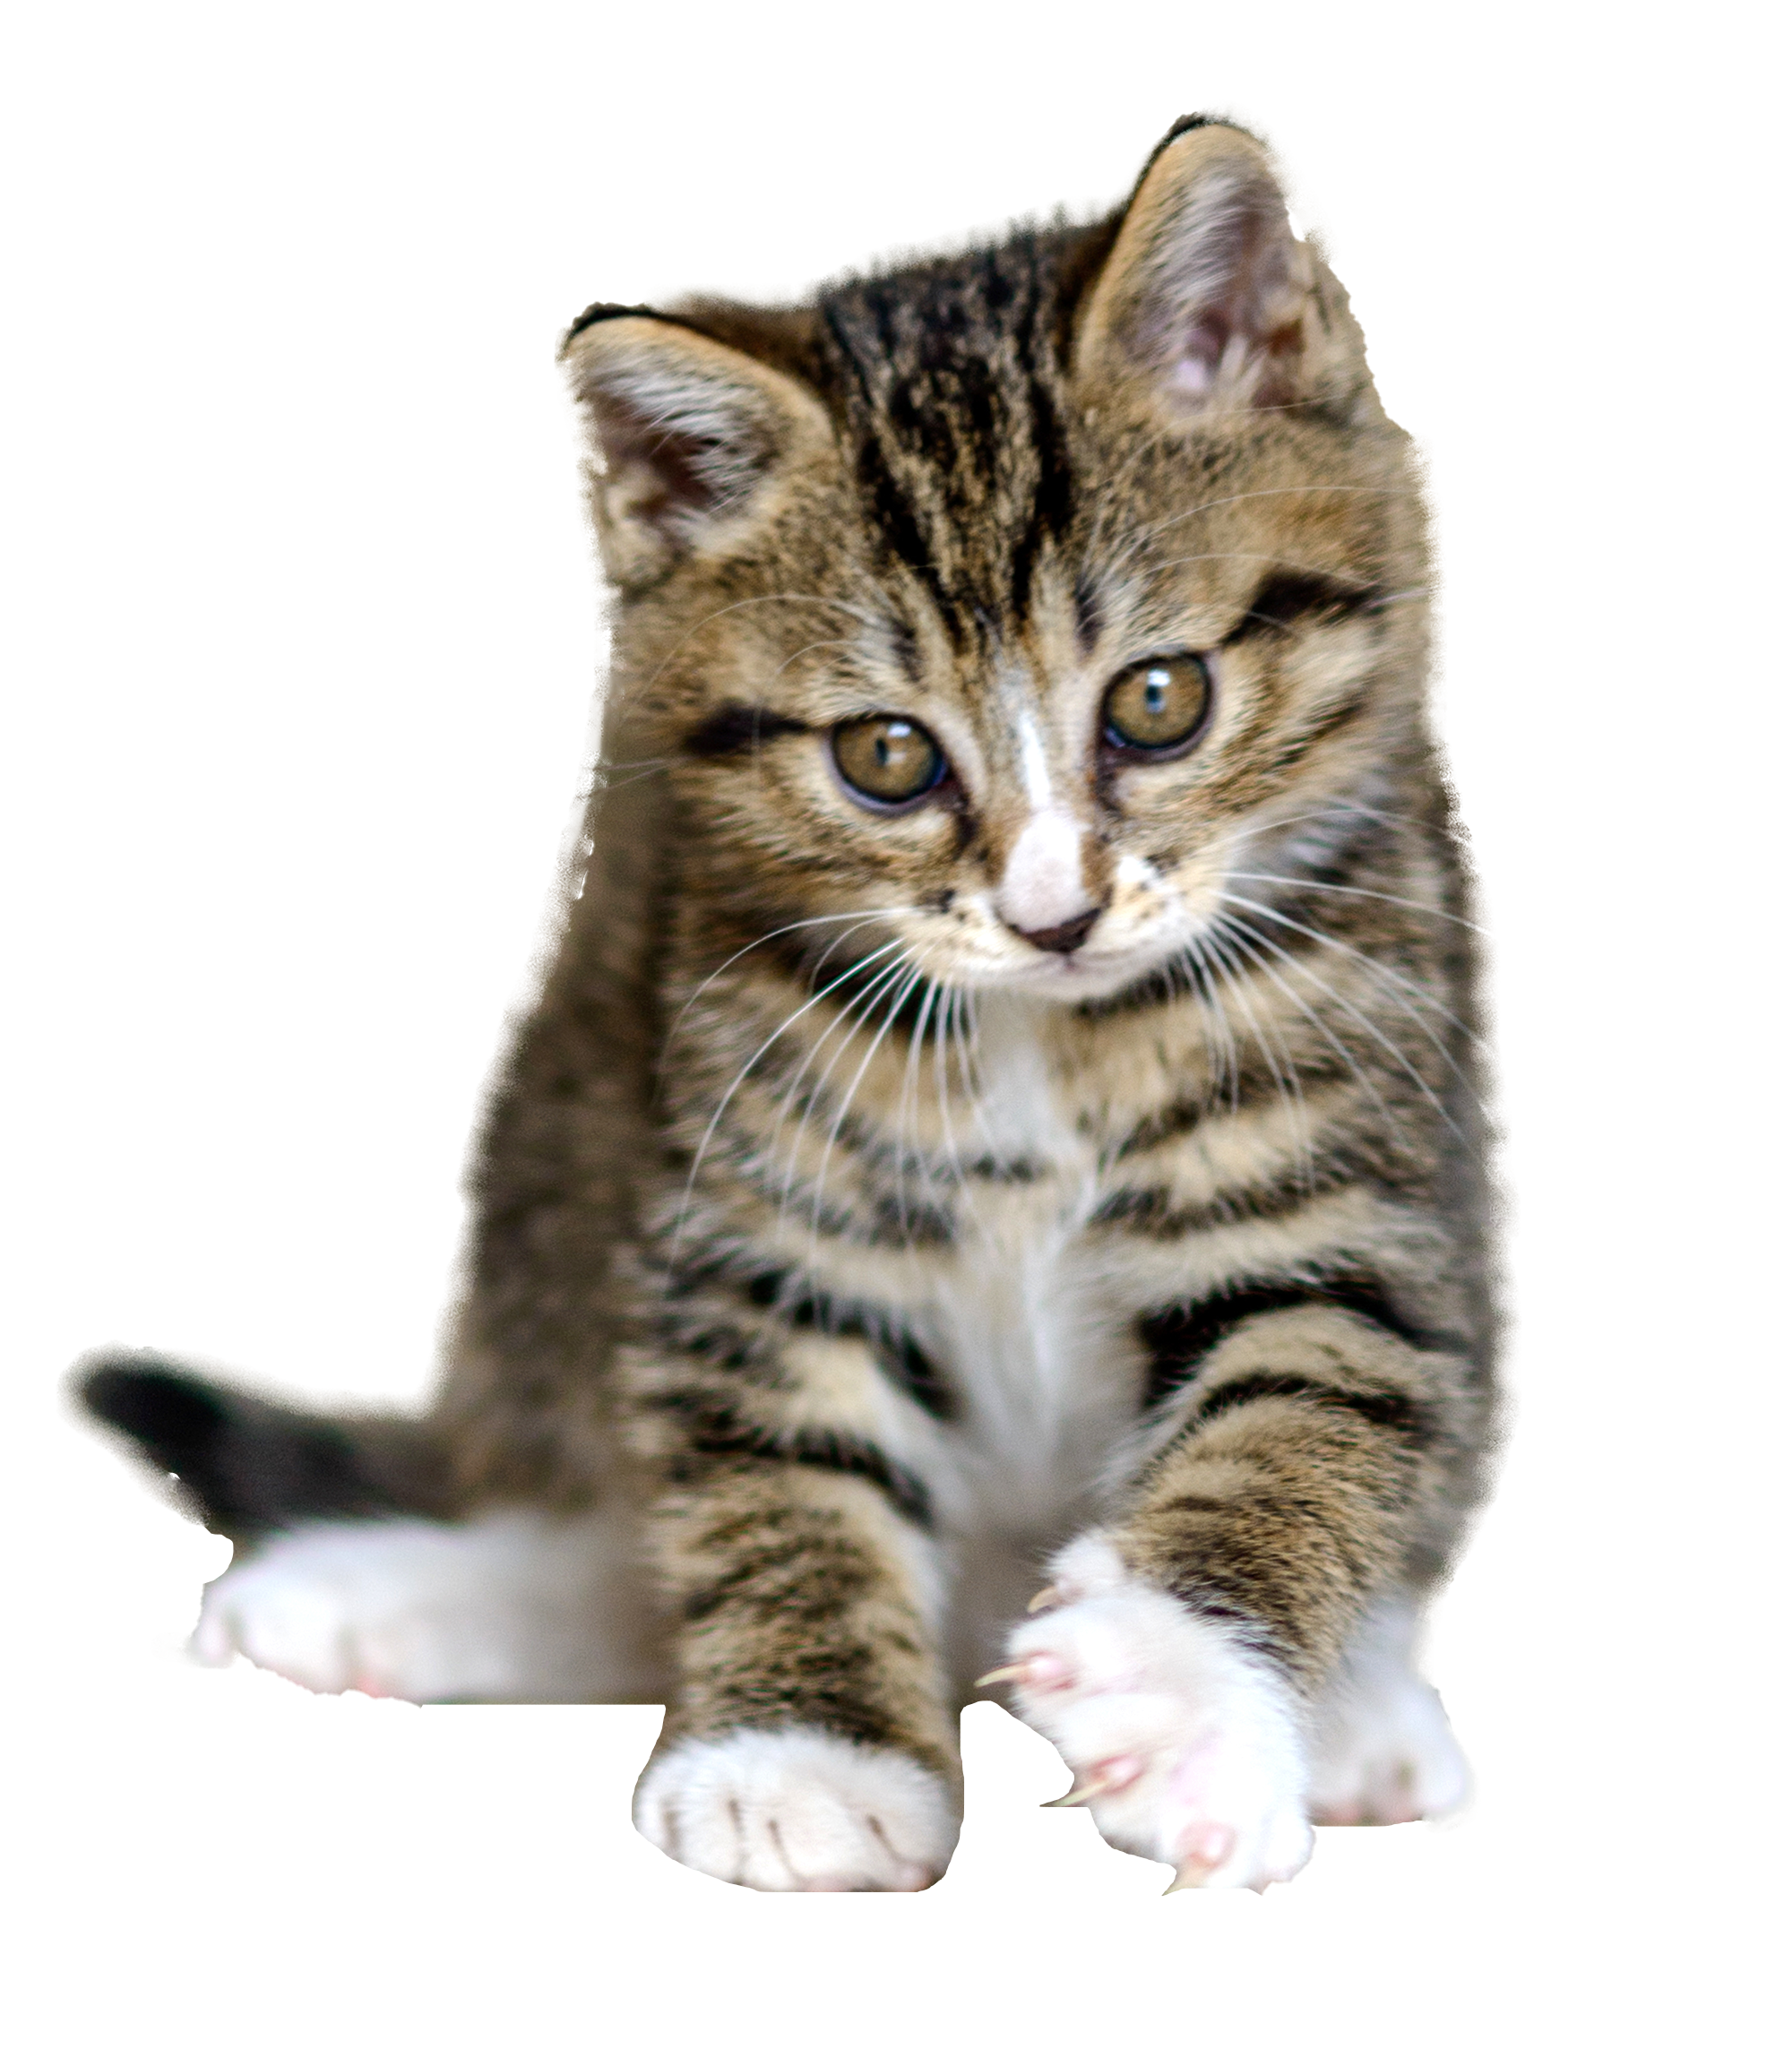
\includegraphics[width=0.7\linewidth]{Figures/images/cat}
        \end{center}
        \begin{center}
             \qquad \qquad 图1
        \end{center}
        \label{fig:tstmp20211203103404}
    \end{figure}
    
}


% 技术领域
\newcommand{\specfield}{
    \begin{large}
        \par 本发明属于小猫领域
    \end{large}
}

% 背景技术
\newcommand{\spectechnology}{
    \begin{large}
        \par 猫行动敏捷,善跳跃。吃鱼、鼠、兔等。猫之所以喜爱吃鱼和老鼠,是因为猫是夜行动物,
        为了在夜间能看清事物,需要大量的牛磺酸,而老鼠和鱼的体内就含牛磺酸,
        所以猫不仅仅是因为喜欢吃鱼和老鼠,也是因为自己的需要才吃。猫作为鼠类的天敌,
        可以有效减少鼠类对青苗等作物的损害,由猫的字形“苗”可见中国古代农业生活之一斑。
    \end{large}
}

\newcommand{\specinvention} {
    \begin{large}
        \par 作为本申请另一实施例,猫能在高墙上若无其事地散步,轻盈跳跃,不禁折服于它的平衡感。
        这主要得益于猫的出类拔萃的反应神经和平衡感。它只需轻微地改变尾巴的位置和高度就可取得身体的平衡,
        再利用后脚强健的肌肉和结实的关节就可敏捷地跳跃,即使在高空中落下也可在空中改变身体姿势,轻盈准确地落地。
        善于爬高,但却不善于从顶点下落。即使从高处掉下或者跳下来的时候,猫靠尾巴调整平衡,使带软垫的四肢着地。
        注意不要拽断猫的尾巴,会影响它的平衡能力,也会容易使猫腹泻,减短猫的寿命。
        \par 作为本申请另一实施例,猫能在高墙上若无其事地散步,轻盈跳跃,不禁折服于它的平衡感。
        这主要得益于猫的出类拔萃的反应神经和平衡感。它只需轻微地改变尾巴的位置和高度就可取得身体的平衡,
        再利用后脚强健的肌肉和结实的关节就可敏捷地跳跃,即使在高空中落下也可在空中改变身体姿势,轻盈准确地落地。
        善于爬高,但却不善于从顶点下落。即使从高处掉下或者跳下来的时候,猫靠尾巴调整平衡,使带软垫的四肢着地。
        注意不要拽断猫的尾巴,会影响它的平衡能力,也会容易使猫腹泻,减短猫的寿命。
        \par 作为本申请另一实施例,猫能在高墙上若无其事地散步,轻盈跳跃,不禁折服于它的平衡感。
        这主要得益于猫的出类拔萃的反应神经和平衡感。它只需轻微地改变尾巴的位置和高度就可取得身体的平衡,
        再利用后脚强健的肌肉和结实的关节就可敏捷地跳跃,即使在高空中落下也可在空中改变身体姿势,轻盈准确地落地。
        善于爬高,但却不善于从顶点下落。即使从高处掉下或者跳下来的时候,猫靠尾巴调整平衡,使带软垫的四肢着地。
        注意不要拽断猫的尾巴,会影响它的平衡能力,也会容易使猫腹泻,减短猫的寿命。
        \par 作为本申请另一实施例,猫能在高墙上若无其事地散步,轻盈跳跃,不禁折服于它的平衡感。
        这主要得益于猫的出类拔萃的反应神经和平衡感。它只需轻微地改变尾巴的位置和高度就可取得身体的平衡,
        再利用后脚强健的肌肉和结实的关节就可敏捷地跳跃,即使在高空中落下也可在空中改变身体姿势,轻盈准确地落地。
        善于爬高,但却不善于从顶点下落。即使从高处掉下或者跳下来的时候,猫靠尾巴调整平衡,使带软垫的四肢着地。
        注意不要拽断猫的尾巴,会影响它的平衡能力,也会容易使猫腹泻,减短猫的寿命。
        \par 作为本申请另一实施例,猫能在高墙上若无其事地散步,轻盈跳跃,不禁折服于它的平衡感。
        这主要得益于猫的出类拔萃的反应神经和平衡感。它只需轻微地改变尾巴的位置和高度就可取得身体的平衡,
        再利用后脚强健的肌肉和结实的关节就可敏捷地跳跃,即使在高空中落下也可在空中改变身体姿势,轻盈准确地落地。
        善于爬高,但却不善于从顶点下落。即使从高处掉下或者跳下来的时候,猫靠尾巴调整平衡,使带软垫的四肢着地。
        注意不要拽断猫的尾巴,会影响它的平衡能力,也会容易使猫腹泻,减短猫的寿命。
        \par 本发明提供的车罩的有益效果在于:猫显得有些任性,我行我素。本来猫是喜欢单独行动的动物,
        不像狗一样,听从主人的命令,集体行动。因而它不将主人视为君主,唯命是从。有时候,你怎么叫它,
        它都当没听见。猫和主人并不是主从关系,把它们看成平等的朋友关系会更好一些。也正是这种关系,
        才显得独具魅力。另一方面猫把主人看作父母,像小孩一样爱撒娇,它觉得寂寞时会爬上主人的膝盖,
        或者随地跳到摊开的报纸上坐着,尽显娇态

    \end{large}
}

\newcommand{\descpic}{
    \begin{large}
        如图1是一只狸花猫,原产于中国,属于自然猫,在宋朝有“狸猫换太子”的故事,
        因此是千百年来经过自然淘汰而保留下来的品种。此猫头圆,面颊宽大,被毛上有漂亮的斑纹,特别容易喂养,并对捕捉老鼠十分在行
    \end{large}
}

\newcommand{\execution}{
    \begin{large}
        附图仅用于示例性说明,不能理解为对本专利的限制;
        为了更好说明本实施例,附图某些部件会有省略、放大或缩小,并不代表实际产品的尺寸;
        对于本领域技术人员来说,附图中某些公知结构及其说明可能省略是可以理解的。
        下面结合附图和实施例对本发明的技术方案做进一步的说明。

        实施例1
        如图1所示,这是一只狸花猫,原产于中国,属于自然猫,在宋朝有“狸猫换太子”的故事,
        因此是千百年来经过自然淘汰而保留下来的品种。此猫头圆,面颊宽大,被毛上有漂亮的斑纹,特别容易喂养,并对捕捉老鼠十分在行

    \end{large}
}


%opening
\begin{document}

	\thispagestyle{empty}

\begin{flushleft}
    \textbf{{\Large(19) 中华人民共和国国家知识产权局}}
\end{flushleft}
\begin{center}
    \textbf{{\LARGE (12)发明专利申请}}
\end{center}

\begin{flushright}
    \textbf{(10)申请公布号}

    \textbf{(43)申请公布日}
    \rule[18pt]{17.3cm}{0.1em}
\end{flushright}
\begin{flushleft}
    \textbf{(21)申请号 }

    \textbf{(22)申请日}

    \textbf{(71)申请人}\quad  xxxx大学

    \hspace{2.5em}\textbf{地址} \quad\hspace{0.5em}330013\quad xxxxxx号


    \textbf{(72)发明人}\quad xxx\quad xxx\quad xxx

    \textbf{(51)int.CI.}

    \quad\quad\textit{\textbf{B60P 1/02}(2006.01)}
\end{flushleft}
\begin{flushright}
%    权力要求书1页 说明书3页 附图2页
    \rule[16pt]{17.3cm}{0.1em}
\end{flushright}

%\rule[16pt]{17.3cm}{0.1em}


\begin{multicols}{2}
    \begin{flushleft}
        \textbf{(54)发明名称}
    \end{flushleft}
    {\large  \name}\\
    \\
    \textbf{(57)摘要}

    \coverabstract
\end{multicols}


	\chead{{\Large \textbf{权利要求书}}}
% 设置页码从1开始
\setcounter{page}{1}

\begin{large}
    1.一种猫装置,其特征在于,包括:
    猫,分多种,是鼠的天敌。各地都有畜养。有黄、黑、白、灰等各种颜色;身形像狸,外貌像老虎,毛柔而齿利(有几乎无毛的品种)。以尾长腰短,目光如金银,上腭棱多的最好。身体小巧,样子招人喜爱。好奇心重。

    2.成年猫咪的牙齿共30枚。幼年猫咪的牙齿共26枚。
    猫的牙齿从两边往中间分别是:
    上排——臼齿大臼齿前臼齿犬齿6颗门齿
    下排——大臼齿前臼齿犬齿6颗门齿

    3.14天左右开始长牙
    2~3周龄乳门牙长齐。近两月龄时,乳牙全部长齐,呈白色,细而尖
    3~4月龄更换第一乳门牙
    5~6月龄换第二三乳门齿及乳犬牙

    4.14天左右开始长牙
    2~3周龄乳门牙长齐。近两月龄时,乳牙全部长齐,呈白色,细而尖
    3~4月龄更换第一乳门牙
    5~6月龄换第二三乳门齿及乳犬牙

    5.14天左右开始长牙
    2~3周龄乳门牙长齐。近两月龄时,乳牙全部长齐,呈白色,细而尖
    3~4月龄更换第一乳门牙
    5~6月龄换第二三乳门齿及乳犬牙

    6.14天左右开始长牙
    2~3周龄乳门牙长齐。近两月龄时,乳牙全部长齐,呈白色,细而尖
    3~4月龄更换第一乳门牙
    5~6月龄换第二三乳门齿及乳犬牙

    7.14天左右开始长牙
    2~3周龄乳门牙长齐。近两月龄时,乳牙全部长齐,呈白色,细而尖
    3~4月龄更换第一乳门牙
    5~6月龄换第二三乳门齿及乳犬牙

    8.14天左右开始长牙
    2~3周龄乳门牙长齐。近两月龄时,乳牙全部长齐,呈白色,细而尖
    3~4月龄更换第一乳门牙
    5~6月龄换第二三乳门齿及乳犬牙

\end{large}

	\newpage
\chead{{\Large \textbf{说明书}}}

\setcounter{page}{1}

\subsection*{
    \begin{center}
        \name
    \end{center}}

\subsection*{技术领域}
\specfield

\subsection*{背景技术}
\spectechnology

\subsection*{发明内容}
\specinvention

\subsection*{附图说明}
\descpic

\subsection*{具体实施方式}
\execution





	\newpage
\chead{{\Large \textbf{说明书 \hspace{1} 附图}}}

\setcounter{page}{1}
\begin{figure}[H]
    \begin{center}
        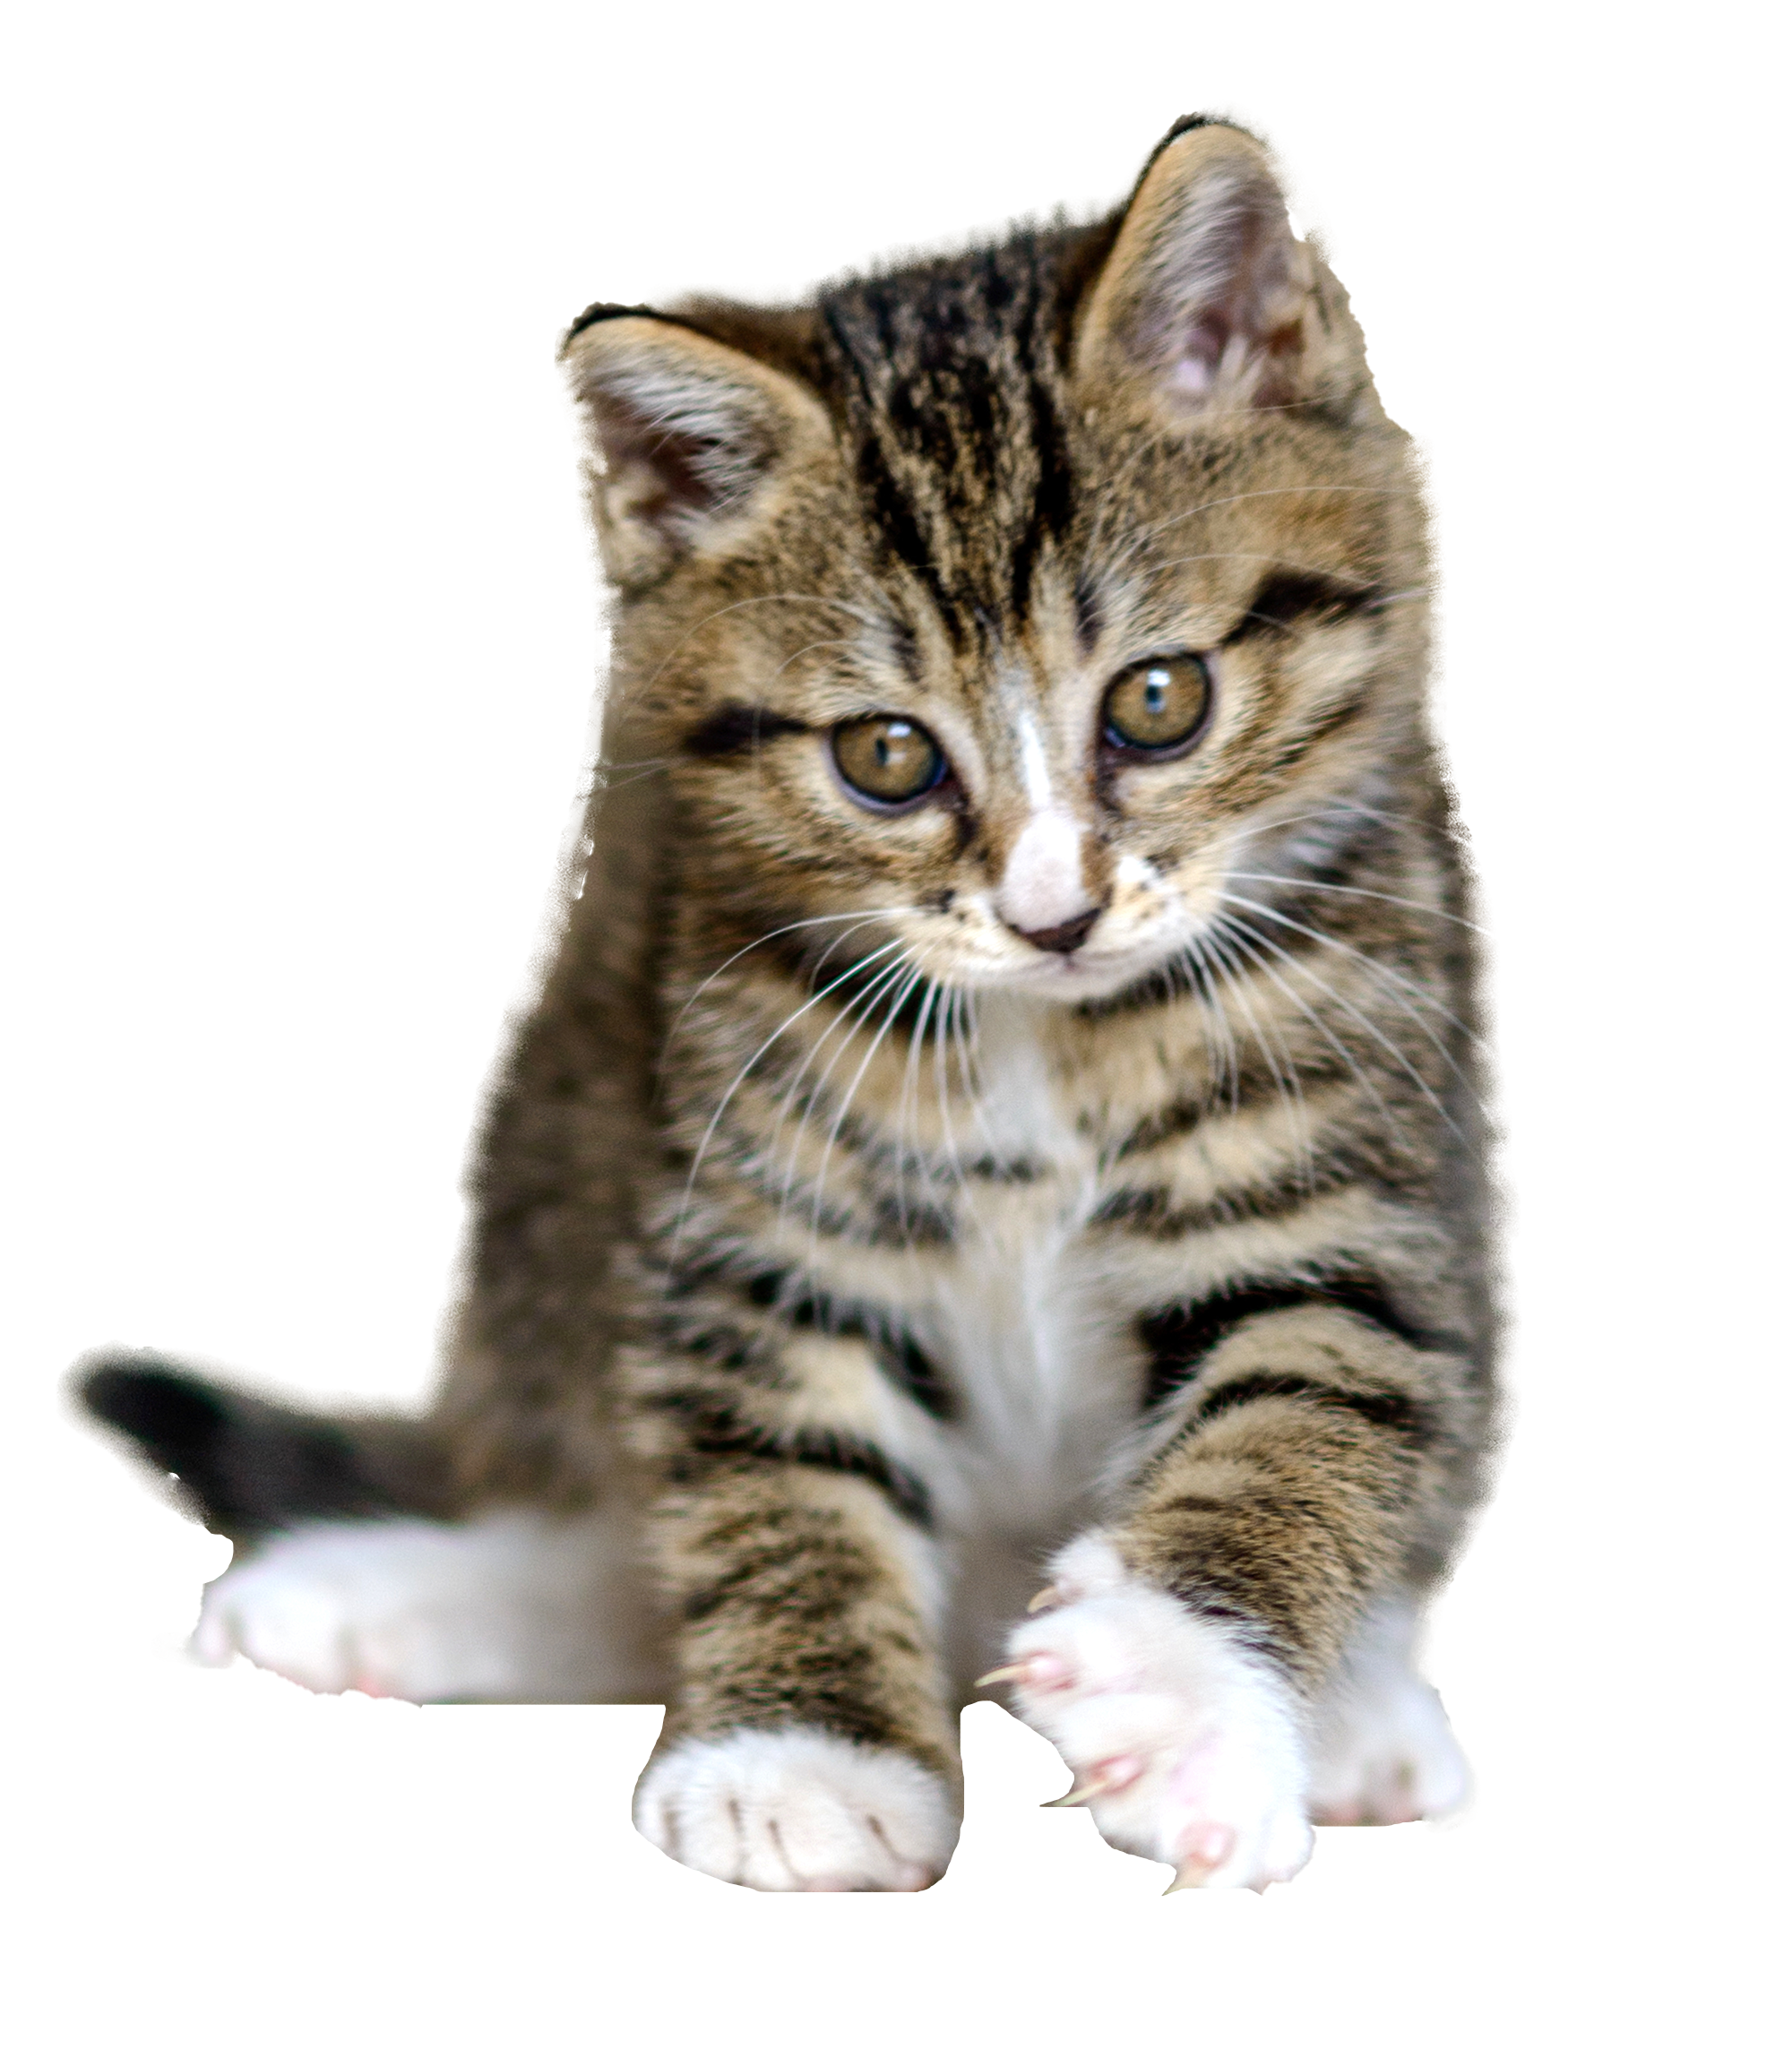
\includegraphics[width=0.7\linewidth]{Figures/images/cat}
    \end{center}
    \begin{center}
        \qquad \qquad 图1
    \end{center}
    \label{fig:tstmp20211203103404}
\end{figure}

\end{document}